\documentclass[tikz, border=12pt]{standalone}

\usepackage{tikz}
\usepackage{amsmath}
\usepackage{amssymb}
\usepackage{bm}
\usepackage{xcolor}
\usepackage{pgfplots}
\pgfplotsset{compat=1.18}
\usepackage[T1]{fontenc}
\usepackage{helvet}
\renewcommand{\familydefault}{\sfdefault}

\usetikzlibrary{
  arrows.meta,
  shapes.geometric,
  positioning,
  fit,
  backgrounds,
  calc,
  decorations.pathreplacing
}

%%─── Colours ──────────────────────────────────────────────────────────────────
\definecolor{panelbg}   {HTML}{F5EFE0}
\definecolor{panelbord} {HTML}{2C2C2A}
\definecolor{tealcol}   {HTML}{1D9E75}
\definecolor{bluecol}   {HTML}{185FA5}
\definecolor{purpcol}   {HTML}{534AB7}
\definecolor{ambrcol}   {HTML}{854F0B}
\definecolor{redcol}    {HTML}{A32D2D}
\definecolor{graycol}   {HTML}{5F5E5A}
\definecolor{nodein}    {HTML}{185FA5}
\definecolor{nodehid}   {HTML}{888780}
\definecolor{nodeout}   {HTML}{3B6D11}
\definecolor{teallight} {HTML}{E1F5EE}
\definecolor{purplight} {HTML}{EEEDFE}
\definecolor{ambrlight} {HTML}{FAEEDA}
\definecolor{greenlight}{HTML}{EAF3DE}

%%─── Styles ───────────────────────────────────────────────────────────────────
\tikzset{
  panel/.style={
    rectangle, rounded corners=7pt,
    fill=panelbg, draw=panelbord, line width=1.0pt,
    inner sep=0pt
  },
  lbl/.style={font=\bfseries\small, text=panelbord, anchor=north west},
  ttl/.style={font=\bfseries\normalsize, text=panelbord, anchor=north},
  neuin/.style ={circle,minimum size=13pt,draw=nodein, fill=nodein!25, line width=0.7pt},
  neuhid/.style={circle,minimum size=11pt,draw=nodehid,fill=nodehid!15,line width=0.5pt},
  neuout/.style={circle,minimum size=13pt,draw=nodeout,fill=nodeout!20,line width=0.7pt},
  fatarrow/.style={
    -{Latex[length=3.5mm,width=2.8mm]},
    line width=2.0pt, color=panelbord},
  stepar/.style={
    -{Latex[length=2.5mm,width=2.0mm]},
    line width=1.2pt}
}

%%──────────────────────────────────────────────────────────────────────────────
\begin{document}
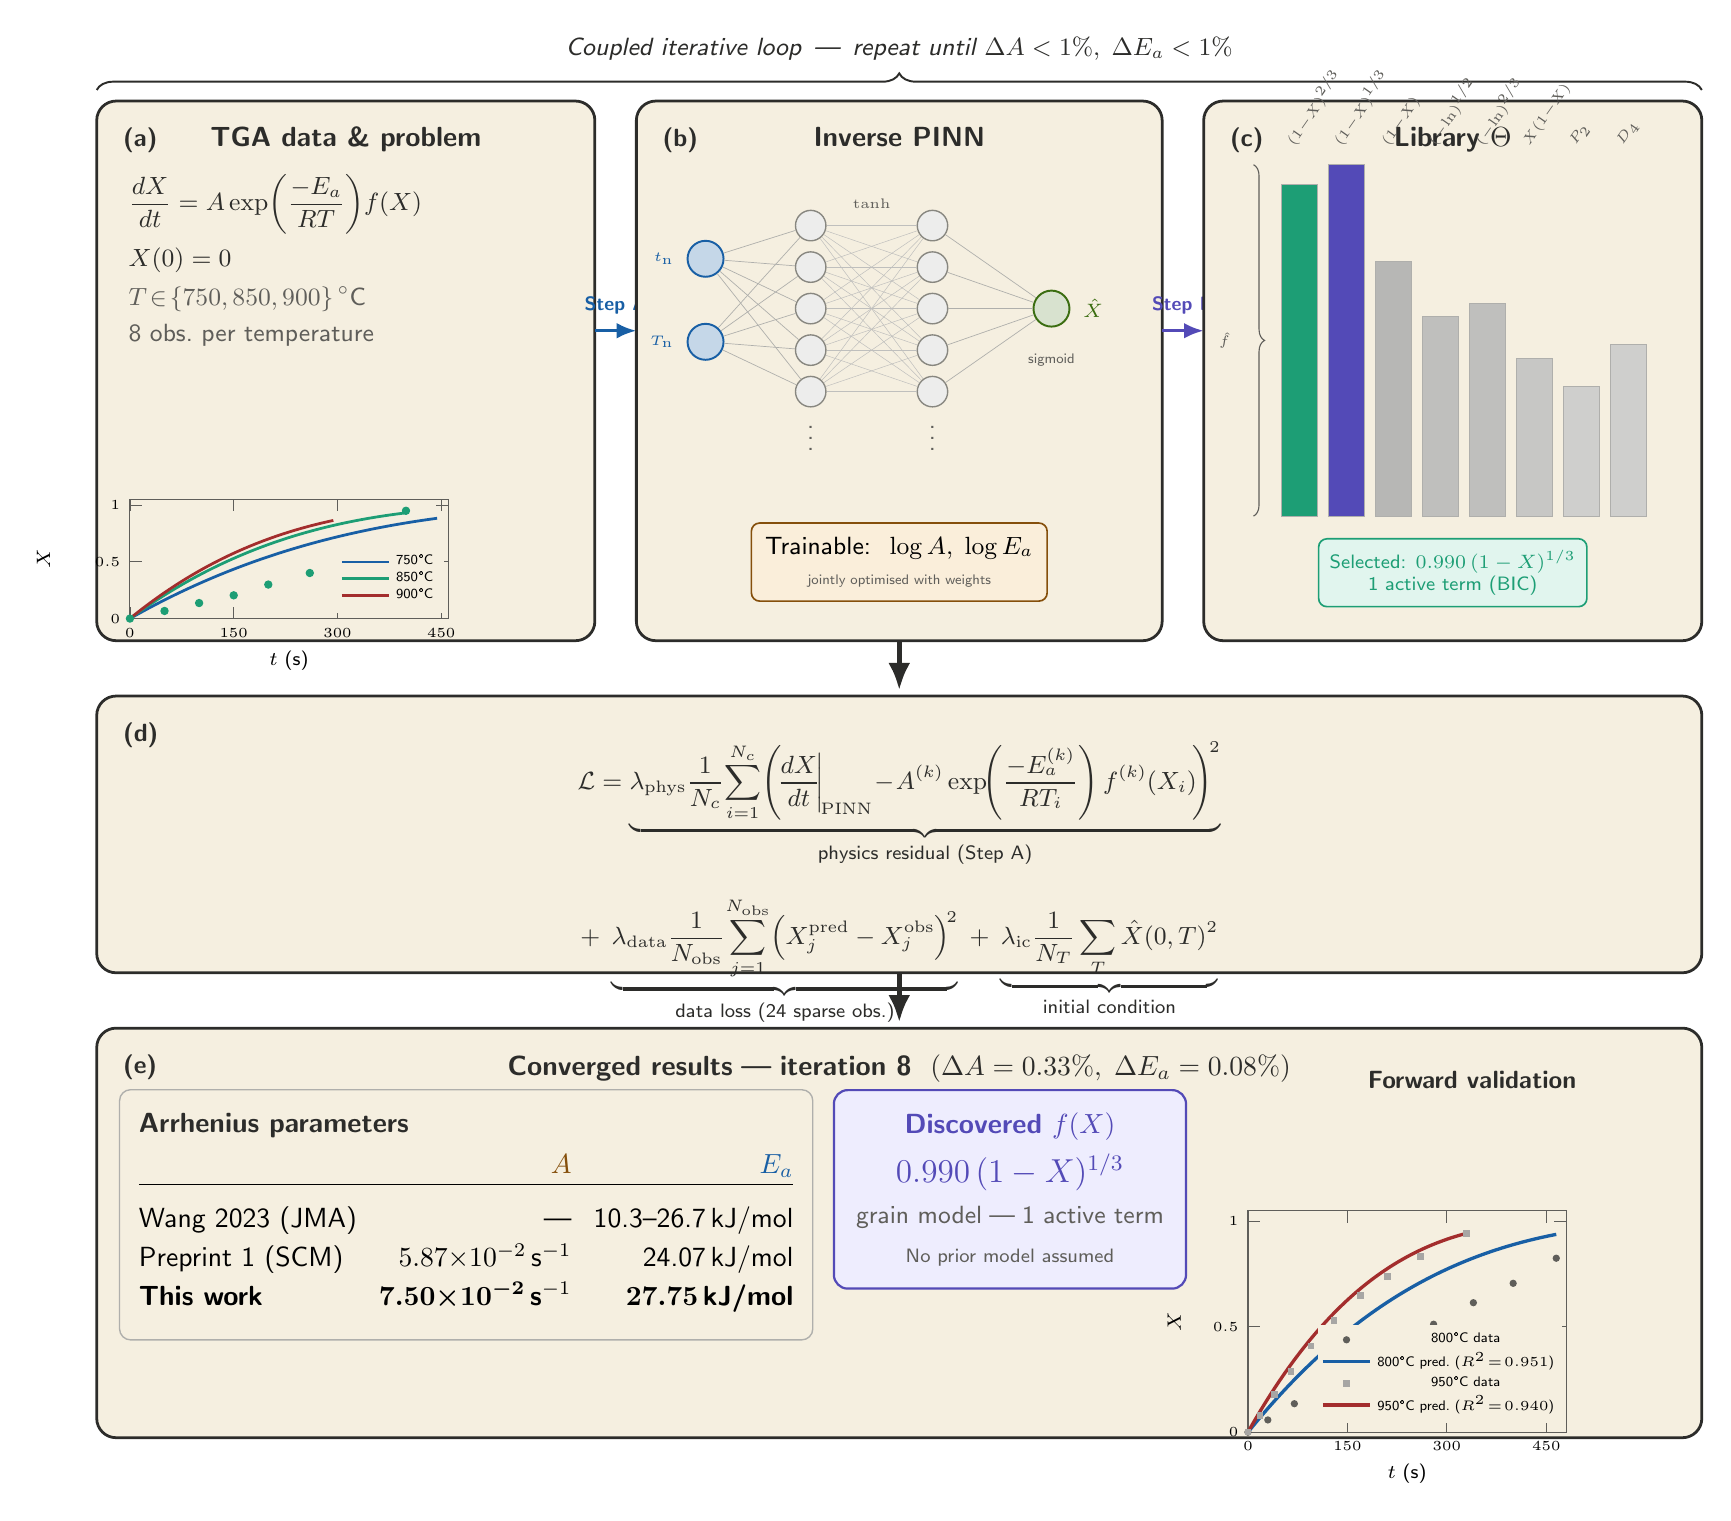
\begin{tikzpicture}[x=1pt,y=1pt]

%%════════════════════════════════════════════════════════════════════════════
%% LAYOUT  (all coordinates in pt)
%%
%%  Top row:
%%    Panel A  x=  0..180   y=  0..195
%%    Panel B  x=195..385   y=  0..195
%%    Panel C  x=400..580   y=  0..195
%%    Total width = 580
%%
%%  Panel D   x=  0..580   y=-120..-20   (height=100, inc. underbrace room)
%%  Panel E   x=  0..580   y=-280..-130  (height=150)
%%
%%  Top brace  y=197..210
%%════════════════════════════════════════════════════════════════════════════

%%──────────────────────────────────────────────────────────────────────────
%%  TOP BRACE + LABEL
%%──────────────────────────────────────────────────────────────────────────
\draw[decorate,
      decoration={brace,amplitude=6pt,raise=2pt},
      color=panelbord,line width=0.7pt]
  (0,197) -- (580,197)
  node[midway,above=9pt,font=\small\itshape,text=panelbord]
  {Coupled iterative loop\enspace---\enspace
   repeat until $\Delta A < 1\%,\;\Delta E_a < 1\%$};

%%──────────────────────────────────────────────────────────────────────────
%%  PANEL (a)   x=0..180   y=0..195
%%──────────────────────────────────────────────────────────────────────────
\draw[panel] (0,0) rectangle (180,195);
\node[lbl] at (6,189) {(a)};
\node[ttl] at (90,189) {TGA data \& problem};

\node[anchor=north west, text=panelbord, align=left, font=\small]
at (8,172)
{$\dfrac{dX}{dt}=A\exp\!\left(\dfrac{-E_a}{RT}\right)\!f(X)$\\[4pt]
 $X(0)=0$\\[3pt]
 \textcolor{graycol}{$T\!\in\!\{750,850,900\}\,^\circ\text{C}$}\\[2pt]
 \textcolor{graycol}{8 obs.\ per temperature}};

%% pgfplots — placed so axis area is strictly inside the panel
%% axis south-west at (12,8), size 160×88
\begin{axis}[
  at={(12pt,8pt)}, anchor=south west,
  width=160pt, height=88pt,
  xlabel={\scriptsize $t$ (s)},
  ylabel={\scriptsize $X$},
  ylabel style={
    at={(axis description cs:-0.22,0.5)},
    anchor=south, rotate=0
  },
  xlabel style={yshift=2pt, font=\scriptsize},
  tick label style={font=\tiny},
  xmin=0,xmax=460,ymin=0,ymax=1.05,
  xtick={0,150,300,450},ytick={0,0.5,1.0},
  axis line style={color=graycol,line width=0.4pt},
  tick style={color=graycol,line width=0.3pt},
  axis background/.style={fill=panelbg},
  legend style={
    font=\tiny,draw=none,fill=panelbg,
    at={(0.99,0.04)},anchor=south east,
    row sep=-3pt,inner sep=2pt},
  clip=true
]
\addplot[bluecol,line width=1.0pt,smooth,domain=0:444,samples=50]
  {1-(max(1-0.00347*x/3,0))^3};
\addlegendentry{750°C}
\addplot[tealcol,line width=1.0pt,smooth,domain=0:399,samples=50]
  {1-(max(1-0.00446*x/3,0))^3};
\addlegendentry{850°C}
\addplot[redcol,line width=1.0pt,smooth,domain=0:294,samples=50]
  {1-(max(1-0.00498*x/3,0))^3};
\addlegendentry{900°C}
\addplot[tealcol,only marks,mark=*,mark size=1.3pt,
         mark options={fill=tealcol}]
  coordinates{(0,0)(50,.067)(100,.137)(150,.205)
               (200,.300)(260,.402)(320,.510)(399,.951)};
\end{axis}

%%──────────────────────────────────────────────────────────────────────────
%%  STEP A ARROW   A→B
%%──────────────────────────────────────────────────────────────────────────
\draw[stepar,bluecol]
  (180,112) -- (195,112)
  node[midway,above=2pt,font=\scriptsize\bfseries,text=bluecol]{Step A};

%%──────────────────────────────────────────────────────────────────────────
%%  PANEL (b)   x=195..385   y=0..195
%%──────────────────────────────────────────────────────────────────────────
\draw[panel] (195,0) rectangle (385,195);
\node[lbl] at (201,189) {(b)};
\node[ttl] at (290,189) {Inverse PINN};

%% Input neurons  x=220
\node[neuin] (in1) at (220,138) {};
\node[neuin] (in2) at (220,108) {};
\node[font=\tiny,text=nodein,anchor=east] at (212,138) {$t_{\mathrm{n}}$};
\node[font=\tiny,text=nodein,anchor=east] at (212,108) {$T_{\mathrm{n}}$};

%% Hidden layer 1  x=258
\foreach \y in {150,135,120,105,90}{
  \node[neuhid] (hA\y) at (258,\y) {};}
\node[font=\small,text=graycol] at (258,76) {$\vdots$};

%% Hidden layer 2  x=302
\foreach \y in {150,135,120,105,90}{
  \node[neuhid] (hB\y) at (302,\y) {};}
\node[font=\small,text=graycol] at (302,76) {$\vdots$};

%% Output  x=345
\node[neuout] (outN) at (345,120) {};
\node[font=\scriptsize,text=nodeout,anchor=west] at (353,120) {$\hat{X}$};
\node[font=\tiny,text=graycol,anchor=north,align=center]
  at (345,107) {sigmoid};

%% Activation label
\node[font=\tiny,text=graycol] at (280,158) {$\tanh$};

%% Connections
\foreach \y in {150,135,120,105,90}{
  \draw[line width=0.25pt,graycol!50] (in1)--(hA\y);
  \draw[line width=0.25pt,graycol!50] (in2)--(hA\y);}
\foreach \ya in {150,135,120,105,90}{
  \foreach \yb in {150,135,120,105,90}{
    \draw[line width=0.18pt,graycol!40] (hA\ya)--(hB\yb);}}
\foreach \y in {150,135,120,105,90}{
  \draw[line width=0.25pt,graycol!50] (hB\y)--(outN);}

%% Trainable box — at the very bottom, clear of neurons
\node[rectangle,rounded corners=3pt,
      fill=ambrlight,draw=ambrcol,line width=0.6pt,
      inner sep=5pt,align=center,font=\small,anchor=south]
at (290,14)
{Trainable:\; $\log A,\;\log E_a$\\
 \textcolor{graycol}{\tiny jointly optimised with weights}};

%%──────────────────────────────────────────────────────────────────────────
%%  STEP B ARROW   B→C
%%──────────────────────────────────────────────────────────────────────────
\draw[stepar,purpcol]
  (385,112) -- (400,112)
  node[midway,above=2pt,font=\scriptsize\bfseries,text=purpcol]{Step B};

%%──────────────────────────────────────────────────────────────────────────
%%  PANEL (c)   x=400..580   y=0..195
%%──────────────────────────────────────────────────────────────────────────
\draw[panel] (400,0) rectangle (580,195);
\node[lbl] at (406,189) {(c)};
\node[ttl] at (490,189) {Library $\Theta$};

%%  8 bars
%%  Bar region: x=420..572,  y=45..172
%%  Available x-width for bars: 152pt
%%  8 bars × 17pt pitch = 136pt → left margin = (152-136)/2 = 8 → start x=428
%%  Each bar: width=13pt, gap=4pt (pitch=17)
%%  Heights (grain model = tallest = 127pt so its top reaches y=172):
%%    (1-X)^(2/3): 120/127 → 120pt
%%    (1-X)^(1/3): 127pt  ← TALLEST (selected)
%%    (1-X)      :  92pt
%%    (-ln)^0.5  :  72pt
%%    (-ln)^(2/3):  77pt
%%    X(1-X)     :  57pt
%%    P2         :  47pt
%%    D4         :  62pt
%%
%%  Bar labels: rotated 55°, placed INSIDE panel, starting at y=175

\def\bstart{428}  %% x of first bar left edge
\def\bboty{45}    %% y of bar base
\def\blabelbase{173} %% y where rotated labels start

%% Colours: 1=teal (SCM), 2=purple (grain=selected), rest=gray
\foreach \i/\ht/\col in {
  1/120/tealcol,
  2/127/purpcol,
  3/92/graycol!45,
  4/72/graycol!40,
  5/77/graycol!40,
  6/57/graycol!35,
  7/47/graycol!30,
  8/62/graycol!30}
{
  \pgfmathsetmacro\bx{\bstart+(\i-1)*17}
  \fill[\col] (\bx,\bboty) rectangle (\bx+13,\bboty+\ht);
  \draw[graycol!50,line width=0.3pt]
    (\bx,\bboty) rectangle (\bx+13,\bboty+\ht);
}

%% Bar labels — placed above bars, rotated, anchored at base so they
%% point rightward and stay inside the panel
\foreach \i/\lbl in {
  1/{$(1{-}X)^{2/3}$},
  2/{$(1{-}X)^{1/3}$},
  3/{$(1{-}X)$},
  4/{$(-\!\ln)^{1/2}$},
  5/{$(-\!\ln)^{2/3}$},
  6/{$X(1{-}X)$},
  7/{$P_2$},
  8/{$D_4$}}
{
  \pgfmathsetmacro\bx{\bstart+(\i-1)*17+6.5}  %% centre of bar
  \node[font=\tiny,text=graycol,
        rotate=55,anchor=south west]
    at (\bx,\blabelbase) {\lbl};
}

%% Left brace
\draw[decorate,decoration={brace,amplitude=4pt},
      color=graycol,line width=0.4pt]
  (418,\bboty+127) -- (418,\bboty)
  node[midway,left=5pt,font=\tiny,text=graycol]{$\hat{f}$};

%% Selected term box
\node[rectangle,rounded corners=3pt,
      fill=teallight,draw=tealcol,line width=0.6pt,
      inner sep=4pt,align=center,font=\scriptsize,text=tealcol,
      anchor=south]
at (490,12)
{Selected: $0.990\,(1-X)^{1/3}$\\1 active term (BIC)};

%%──────────────────────────────────────────────────────────────────────────
%%  FAT ARROW  top row → panel D
%%──────────────────────────────────────────────────────────────────────────
\draw[fatarrow] (290,0) -- (290,-18);

%%──────────────────────────────────────────────────────────────────────────
%%  PANEL (d)   x=0..580   y=-120..-20   height=100
%%──────────────────────────────────────────────────────────────────────────
\draw[panel] (0,-120) rectangle (580,-20);
\node[lbl] at (6,-26) {(d)};

%% Loss formula — two-line layout, centred in panel
%% Line 1 top at y=-30, line 2 below
\node[anchor=north,text=panelbord,align=center,font=\small]
at (290,-33)
{$\mathcal{L}=
\underbrace{%
  \lambda_{\mathrm{phys}}
  \dfrac{1}{N_c}\!\sum_{i=1}^{N_c}
  \!\left(\!
    \dfrac{dX}{dt}\!\bigg|_{\!\mathrm{PINN}}
    \!-\!A^{(k)}\exp\!\!\left(\dfrac{-E_a^{(k)}}{RT_i}\right)
    f^{(k)}(X_i)
  \!\right)^{\!2}
}_{\text{\scriptsize physics residual (Step A)}}$
\\[10pt]
$+\;
\underbrace{%
  \lambda_{\mathrm{data}}
  \dfrac{1}{N_{\mathrm{obs}}}\!\sum_{j=1}^{N_{\mathrm{obs}}}
  \!\left(X_j^{\mathrm{pred}}-X_j^{\mathrm{obs}}\right)^{\!2}
}_{\text{\scriptsize data loss (24 sparse obs.)}}
\;+\;
\underbrace{%
  \lambda_{\mathrm{ic}}
  \dfrac{1}{N_T}\sum_{T}\hat{X}(0,T)^2
}_{\text{\scriptsize initial condition}}$
};

%%──────────────────────────────────────────────────────────────────────────
%%  FAT ARROW  panel D → panel E
%%──────────────────────────────────────────────────────────────────────────
\draw[fatarrow] (290,-120) -- (290,-138);

%%──────────────────────────────────────────────────────────────────────────
%%  PANEL (e)   x=0..580   y=-288..-140   height=148
%%──────────────────────────────────────────────────────────────────────────
\draw[panel] (0,-288) rectangle (580,-140);
\node[lbl] at (6,-146) {(e)};
\node[ttl] at (290,-146)
  {Converged results\;---\;iteration 8\;
   $(\Delta A=0.33\%,\;\Delta E_a=0.08\%)$};

%%── Left: Arrhenius table   x=8..225 ─────────────────────────────────────
%%  Table placed anchored at NW = (8,-162)
\node[rectangle,rounded corners=4pt,
      fill=panelbg,draw=graycol!50,line width=0.5pt,
      inner sep=7pt,anchor=north west]
at (8,-162)
{%
\setlength{\tabcolsep}{4pt}%
\begin{tabular}{@{}l r r@{}}
\multicolumn{3}{@{}l}
  {\textbf{\textcolor{panelbord}{Arrhenius parameters}}}\\[3pt]
 & \textcolor{ambrcol}{$A$} & \textcolor{bluecol}{$E_a$}\\
\hline\\[-5pt]
Wang 2023 (JMA)
  & ---
  & 10.3--26.7\,kJ/mol\\[2pt]
Preprint 1 (SCM)
  & $5.87{\times}10^{-2}\,\text{s}^{-1}$
  & 24.07\,kJ/mol\\[2pt]
\textbf{This work}
  & $\bm{7.50{\times}10^{-2}}\,\textbf{s}^{-1}$
  & $\bm{27.75}$\,\textbf{kJ/mol}\\[2pt]
\end{tabular}%
};

%%── Centre: Discovered f(X)   centred at x=330 ───────────────────────────
\node[rectangle,rounded corners=5pt,
      fill=purplight,draw=purpcol,line width=0.8pt,
      inner sep=8pt,align=center,anchor=north]
at (330,-162)
{%
\textbf{\textcolor{purpcol}{Discovered $f(X)$}}\\[4pt]
\textcolor{purpcol}{\large$0.990\,(1-X)^{1/3}$}\\[3pt]
\textcolor{graycol}{\small grain model\;---\;1 active term}\\[2pt]
\textcolor{graycol}{\scriptsize No prior model assumed}%
};

%%── Right: Forward validation plot   x=415..574   y=-148..-148-130=-278 ──
%%  axis south-west at (416,-286), size=160×128
\node[font=\small\bfseries,text=panelbord,anchor=north]
  at (497,-152) {Forward validation};

\begin{axis}[
  at={(416pt,-286pt)}, anchor=south west,
  width=160pt,height=125pt,
  xlabel={\scriptsize $t$ (s)},
  ylabel={\scriptsize $X$},
  ylabel style={
    at={(axis description cs:-0.18,0.5)},
    anchor=south,rotate=0
  },
  xlabel style={yshift=2pt,font=\scriptsize},
  tick label style={font=\tiny},
  xmin=0,xmax=480,ymin=0,ymax=1.05,
  xtick={0,150,300,450},ytick={0,0.5,1.0},
  axis line style={color=graycol,line width=0.4pt},
  tick style={color=graycol,line width=0.3pt},
  axis background/.style={fill=panelbg},
  legend style={
    font=\tiny,draw=none,fill=panelbg,
    at={(0.99,0.04)},anchor=south east,
    row sep=-2pt,inner sep=1pt},
  clip=true
]
%% 800°C data
\addplot[graycol,only marks,mark=*,mark size=1.1pt,
         mark options={fill=graycol}]
  coordinates{(0,0)(30,.058)(70,.135)(120,.228)(170,.321)
               (220,.408)(280,.512)(340,.614)(400,.706)(465,.825)};
\addlegendentry{\tiny 800°C data}
\addplot[bluecol,line width=1.2pt,smooth,domain=0:465,samples=40]
  {1-(max(1-0.0039*x/3,0))^3};
\addlegendentry{\tiny 800°C pred.\ ($R^2\!=\!0.951$)}
%% 950°C data
\addplot[graycol!55,only marks,mark=square*,mark size=1.0pt,
         mark options={fill=graycol!55}]
  coordinates{(0,0)(18,.080)(40,.178)(65,.288)(95,.408)
               (130,.530)(170,.648)(210,.738)(260,.832)(330,.941)};
\addlegendentry{\tiny 950°C data}
\addplot[redcol,line width=1.2pt,smooth,domain=0:330,samples=40]
  {1-(max(1-0.0056*x/3,0))^3};
\addlegendentry{\tiny 950°C pred.\ ($R^2\!=\!0.940$)}
\end{axis}

\end{tikzpicture}
\end{document}